%==================================================================================================
\chapter{Neural networks}
\FloatBarrier

In this chapter attention will be given to artificial neural networks (ANN) which are one of most 
popular data processing models in self learning systems \cite{Abiodun2019} \cite{Tran2021}
\cite{Syed2021}. First focus will be given to biological neural networks, that will be referred 
to as a neural circuits (NC) in order to be consistent with nomenclature \cite{Purves2001} as 
well as to avoid confusion with ANN.  
After that an electrical models of NC will be shortly described and finally a mathematical models
that are used in modern ANN solutions will be discussed. Special attention will be given to 
computational complexity of both running and teaching described ANN models. 



%==================================================================================================
\section{Neural circuits in biological systems}
\FloatBarrier
In case of organic systems two kinds of information processing subsystems can be distinguished
\cite{Johnson2016}:
\begin{itemize}
	\item neural system which is low latency localized signal processing system that requires
	both source and sink of signal to be directly connected to it, 
	\item endocrine system which is high latency system that influences whole organism and do 
	not require direct connection to affected cells as information is delivered in form of 
	hormones in blood.
\end{itemize}
While both systems interact witch each other and are important for correct functioning of 
organisms \cite{Schwarz2019} in this work attention will be given only to neural system with
special focus on interneurons that process already collected data.


%--------------------------------------------------------------------------------------------------
\subsection{Neural cell as a base of information processing circuit}
\FloatBarrier
At most basic level a neuron is an animal cell which means it must contain all organelle that
are common among those type of cells as well as be able to realize most of metabolic processes.
\begin{figure}[htb] 
	\centering
	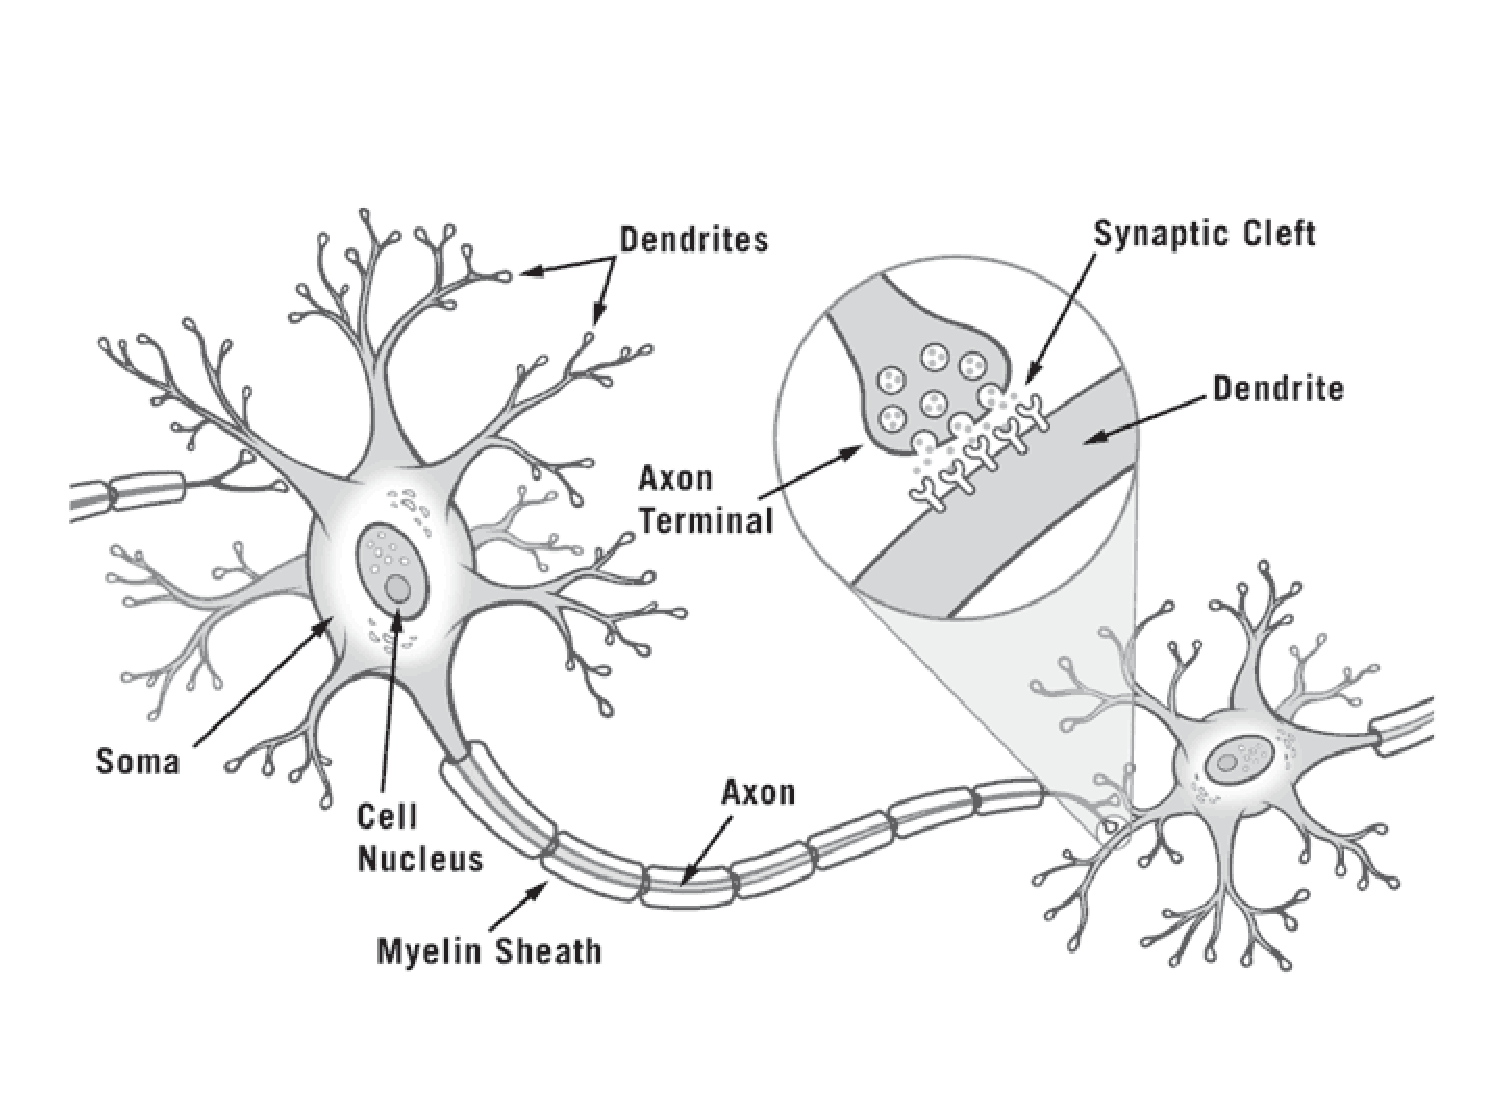
\includegraphics[width=0.8\textwidth]{figures/neural_cell}
	\caption{Structure of a neural cell \cite{Cook2014}}
	\label{fig:neural_cell}
\end{figure}
While all parts of cell are required for its function it is not aim of this work to describe 
cell biology, as such only elements that are directly involved in neurotransmission will be
described in more detail as shown on Figure \ref{fig:neural_cell}.
Soma, also called a cell body, contains nucleus with genetic material and is considered the 
tropic center of a neural cell \cite{Jacobson2017}. From it extend dendrites that increase a 
receptive surface of  the neuron.
At place called axon hillock an single elongated appendix, called axon, protrudes
from a cell body. Its role is to transmit neuron response as a electrical signal into another
cells. In order to correctly carry out this function axon must be protected from environment 
by a myelin sheath. Those sheaths are not integral part of the neuron and are created by a
Schwann cells in peripheral nervous system and by a glial cells in central nervous system.
Area of contact between axon of one nerve cell and dendrites of another is called synapse.
There are two basic types of synapses:
\begin{itemize}
	\item Electrical synapses that are connected with membrane bridges and gap junctions
	that allow direct transmission of electrical impulse between the cells \cite{Connors2017}.
	Those synapses have negligible latency and risk of misfiring.
	Electrical synapses are most commonly found in fish \cite{Yao2014}, however they also appear
	to some degree in mammalian brains \cite{Connors2004}.
	\item Chemical synapses that contain vesicles on presynaptic side and membrane receptors on 
	postsynaptic \cite{Fuster2015}.
	The neurotransmitter released by the action potential is exocytosed and diffuses
	across the synaptic cleft and binds to the specific receptor on the postsynaptic membrane.
	Most of the synapses seen in the mammalian central nervous system are chemical \cite{Boto2019}.
\end{itemize}
The way in which signal processing in neuron occurs starts with neurotransmitters released by
postsynaptic sides of other neurons reaching receptors on dendrites which causes electrical
potential on soma to change. Under neutral condition electrical potential of cell membrane is 
maintained at $-70 mV$ and is referred to as resting potential \cite{Tadeusiewicz1994}. 
How much that potential changes depends on two factors, amount of neurotransmitter released by 
other neuron and type as well as  amount of receptors on neuron which potential is modified.
Number of neurotransmitters is synonymous with input signal strength while receptor type and count
can be understood as a  weight assigned to given connection.
Those weight can be either positive in which case such connection is called excitatory or negative 
for inhibitory connections. 
Receptor configuration is what determines individual neuron transfer function and defines it as 
a signal processing unit.  
\begin{figure}[htb] 
	\centering
	
\includegraphics[width=0.8\textwidth]{figures/bio_activation}
	\caption{Membrane potential of neural cell \cite{Verber2012}}
	\label{fig:bio_activation}
\end{figure}
Effects of all synapses sum up and moderate neuron electrical potential that until action 
potential is reached will return to resting potential after neurotransmitter will no longer
be present \cite{Osowski1994}. However if action potential is reached neuron polarization almost
instantly changes to $30 mV$, such event is referred to as neuron activation. 
This state lasts for a very short time, less than microsecond, and after that neuron enters
refractory period in which membrane potential drops bellow resting potential and cell cannot
be activated. Such process of singleactivation is visualised by a plot on Figure 
\ref{fig:bio_activation}. As long as neurotransmitters are still present at neuron dendrites when
refractory period ends cell will once again activate.
Activation causes neuron to release its own neurotransmitters at end of its axon and so signal
can propagate over multiple neurons. 

